\chapter{Methodology}\label{chapter:methodology}

\begin{figure}
	\centering
	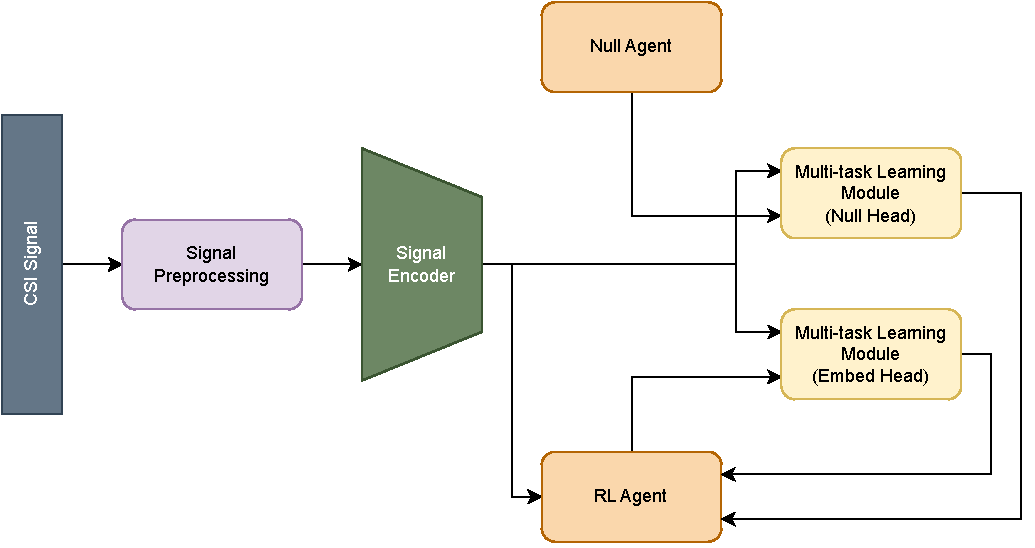
\includegraphics[width=\linewidth]{figures/arch_diagram.pdf}
	\caption{An abstracted diagram of the proposed architecture in this thesis. Red-brown components are for signal processing and signal-to-image transformation. Green components are for the signal encoding, yellow components are the multi-task-learning modules, orange components are for RL, and blue components are either input or outputs of the model.}
	\label{fig:arch-diagram}
\end{figure}

The general intuition behind our approach is the lack of ability for a model to perform on unseen domains without any additional information.
The general architecture of our approach can be seen in Figure \ref{fig:arch-diagram}.
We first propose a signal preprocessing and signal-to-image transformation pipeline, described in Section \ref{sec:methodology-signal-preprocessing} and \ref{sec:methodology-signal-to-image}.
This transforms the input signal into an image that is then passed through a CNN encoder, as described in Section {sec:methodology-signal-encoding}, encoding the signal into a latent representation.
This latent representation is then used in two different ways: As an input for the multi-task learning heads, described in Section \ref{sec:methodology-multi-task-learning}, and as the state observation for our RL agent.

Two mitigate domain-shift, our RL agent is tasked with producing the best possible embedding of the domain $D_{r}$ as its action given the signal latent representation as its state observation.

To provide the RL agent with a reward function, inspired by triplet loss, we use two different multi-task learning modules.
One of these modules is provided $D_{0}$, representing a vector of zeros, and the other $D_{r}$.

\todonotestodo[inline]{This chapter is not finalized, due to the possibility of changing things around so will be kept as bullet points at this stage.}

\section{Signal Processing}\label{sec:methodology-signal-preprocessing}

As the old adage goes, garbage in, garbage out.
As such, we propose the following steps from traditional signal processing to clean up the input signal for our ML algorithm.

\begin{itemize}
	\item Noise filtering with a low-pass filter, since high-freq noise is most likely not human movement
	\item CSI Phase unwrapping and linear fitting as suggested by \cite{geng2022densepose}
	\item CSI Phase derivative, to keep values from changing magnitude as in the case of unwrapping
	\item DWT seems to have been attempted in some papers, so let's see if that helps.
	\item We'll do an ablation study to see if these actually help
\end{itemize}

\section{Signal-to-Image Transformation}\label{sec:methodology-signal-to-image}

Four crazy signal-to-image transformation methods! You won't believe number three!\todo{If there are no objections, this will be in the final paper}

As we wish to leverage advances from computer vision in our algorithm, we must first transform the signal into an image.
There are many works from the literature which show that there are certainly improvements that can be gained from performing image processing on temporal data.
We will experiment with the following four methods for signal-to-image transformation: DeepInsight \cite{sharma2019deepinsight}, REFINED \cite{bazgir2020representation}, GAF/FGAF (Feature-wise GAF) \cite{wang2015imaging,satyawan2023cnns}, and MTF \cite{wang2015imaging}.

\subsection{DeepInsight}

DeepInsight \cite{sharma2019deepinsight} applies t-SNE on the columns of $V$, resulting in each AP $k$ being mapped to a point in 2D space.
The entire space is then rotated to fit within the minimum rectangular bounding box.
These rotated points then become the pixel coordinates for a given AP.
The value of the RSSI of a given AP $k$ is then directly mapped to the value of its corresponding pixel.
If multiple features share a pixel location, the average value of these features is then used as the value of the pixel.

\subsection{REFINED}

REpresentation of Features as Images with NEighborhood Dependencies \cite{bazgir2020representation} uses a technique the authors call ``Bayesian Multidimensional Scaling''.
A 2D embedding of the data $V_{embed}$ is calculated using Multidimensional Scaling (MDS) with a Euclidean distance metric.
A pixel grid $P$ of $p^2$ pixels, where $p=\left\lceil \sqrt{K} \right\rceil$ is then produced with dimensions $p \times p$.
A mapping of features to pixels is calculated by considering all permutations which minimize the Euclidean distance of the pixel mapping to the feature location in $V_{embed}$ while keeping at most one feature per pixel iteratively.
This final mapping is calculated using a hill-climb algorithm.

\subsection{GAF}

Gramian Angular Fields \cite{wang2015imaging} first transform the incoming signal for each AP to polar coordinates with
\begin{equation}
	\vec{w_{i, k}} = \begin{cases}
		\phi_{i, k} = \arccos(V_{n, k}) \\
		r_{i, k} = i / I
	\end{cases}
\end{equation}
where $\vec{w_{i, k}}$ is the resulting vector of a signal, $V_{i, k}$ the value of the signal from AP $K$ at sample $i$, $i$ the sample number of the fingerprint, and $I$ the total number of timesteps at the given sample location.
For the case of our dataset, there are 6 timesteps for each location.

The Gramian is than calculated as
\begin{equation}
	G_k = \begin{bmatrix}
		w_{1,k} \cdot w_{1,k} & \cdots & w_{1,k} \cdot w_{I,k} \\
		\vdots                & \ddots & \vdots \\
		w_{I,k} \cdot w_{1,k} & \cdots & w_{I,k} \cdot w_{I,k}
	\end{bmatrix}
\end{equation}
for each AP $k$ creating an image with $k$ channels.

We discovered in a previous project that calculating vector $\vec{w}$ across features, i.e., channels, instead of across timesteps can also be useful. 
This results in
\begin{equation}
	\vec{w_{n, k}} = \begin{cases}
		\phi_{n, k} = \arccos(V_{n, k}) \\
		r_{n, k} = k / K
	\end{cases}
\end{equation}
where $n$ is the sample index and $k$ is the feature index. This leads to the Gramian for each sample 
\begin{equation}
	G_n = \begin{bmatrix}
		w_{n, 1} \cdot w_{n, 1} & \ldots & w_{n, 1} \cdot w_{n, K} \\
		\vdots                  & \ddots & \vdots \\
		w_{n, K} \cdot w_{n, 1} & \cdots & w_{n, K} \cdot w_{n, K}
	\end{bmatrix}
\end{equation}
We call this transformation Feature-wise GAF (FGAF).

In either case, $G$ is finally normalized.

\subsection{MTF}
Markovian Transition Fields \cite{wang2015imaging} first quantizes the signal into $q$ bins, each bin representing an interval of RSSI strength.
A Markovian transition matrix $M_{t}$ is then constructed where each row represents a fingerprint and each column a bin. 
The values in $M_{t}$ are the size of each bin for a given sample.
$M_{t}$ is then normalized and aligned along the temporal axis such that in this new matrix $M$, $M_{i, j}$ represents the probability of a transition from bin $i$ to bin $j$.
$M$ is then an image of size $q \times q$.

\section{Signal encoding}\label{sec:methodology-signal-encoding}

Once the signal has been transformed into an image, we then calculate a latent representation using a CNN.

\begin{itemize}
	\item The signal encoding backbone is a standard CNN
	\item This will probably be something simple, like ResNet since the signal shouldn't be too complex that it requires something very SOTA
	\item Alternatively, mobilenet may be used as well
	\item This may actually be the least important aspect of this thesis
\end{itemize}

\section{Unsupervised Domain Representations through Reinforcement Learning}

To mitigate domain shift, we implement a novel method for unsupervised domain representations through reinforcement learning.

\begin{itemize}
	\item Base terminology: Agent, action, state observation (state), and reward
	\item The encoder-decoder architecture described in Section \ref{sec:methodology-signal-encoding} and \ref{sec:methodology-multi-task-learning} is the environment.
	\item RL loop:
	\begin{enumerate}
		\item The agent receives the image embedding produced by the encoder/backbone as its state
		\item The reinforcement learning agent produces an embedding of the domain as its action
		\item The environment is trained with one pair of heads receiving the action of the agent while the other pair receives senseless values (either all 0s if the representation is one-hot or a uniform distribution if the representation is a probability measure)
		\item After training of the agent, the RL agent is provided a reward from the environment which is used to improve the agent
	\end{enumerate}
	\item Let the loss function $\mathcal{L}_{w}, \mathcal{L}_{wo}$ represent the loss function of the heads with and without the action provided by the agent, respectively
	\item Then, the reward function $\mathcal{R}$ of the agent is $\mathcal{R} = \mathcal{L}_{wo} - \mathcal{L}_{w}$
	\begin{itemize}
		\item The intuition is, the reward is based on how much better the head pair with the action should perform than the head pair without the action
	\end{itemize}
	\item To speed up training, we take a page from AutoML competitions and the environment is trained within 1 minute and be focused on improving performance as fast as possible instead of achieving the best performance, at least during hyperparam optimization
	\item After hyperparameters are chosen, then we train properly and fully.
	\item A reward is then calculated using the function $R\left(M\left(\hat{y}_{rl}, y\right)-M\left(\hat{y}_{0}, y\right)\right)$, where $M$ is the metric used to calculate the performance of the gesture classifier in each multi-task learning module and $R$ is some reward function.
	\item We do not use the absolute difference, as we are interested in the having negative values representing the module provided $D_0$ having better performance.
\end{itemize}

\section{Multi-task Learning}\label{sec:methodology-multi-task-learning}

The actual gesture classification module is built using a multi-task learning module.

\begin{itemize}
	\item The idea is to enforce some sort of representation that \textit{can} be used to get a domain-independent representation of the data
	\item We utilize multi-task learning for this, where one head is used to predict BVP, which is theoretically domain-independent \cite{zheng2019zero}
	\item The other head is a classifier head and classifies gestures
	\item It's been shown that doing multi-task learning like this leads to good results with latent representations which are more robust \cite{tuggener2021deepscoresv2}
	\item We duplicate this pair of heads to enable a reward function for the RL agent inspired by triplet loss
\end{itemize}
